\chapter{Specification}\label{ch:specification}

During the thesis project, my main task is to design an e-learning platform that offers personalized learning experiences using large language models and spaced repetition learning algorithms. The platform generates questions for the selected question type after users submit their learning materials as a context. Afterward, users can learn from them using the built-in spaced repetition learning algorithm.

After the design phase, I must implement a prototype using modern web technologies like the Go language, Echo backend framework, and HTMX frontend. The platform must integrate a large language model capable of generating questions and use a repetition algorithm to schedule the user-selected questions.

The prototype must run on the web and be accessible from Chromium-based browsers such as Chrome, Edge, and Arc. The features are available for registered users after authentication.

\section{Use cases}

I will describe the use cases of the planned features on the platform below. Figure~\ref{fig:use-case} shows the use-case diagram of the platform.

\begin{figure}[H]
    \centering
    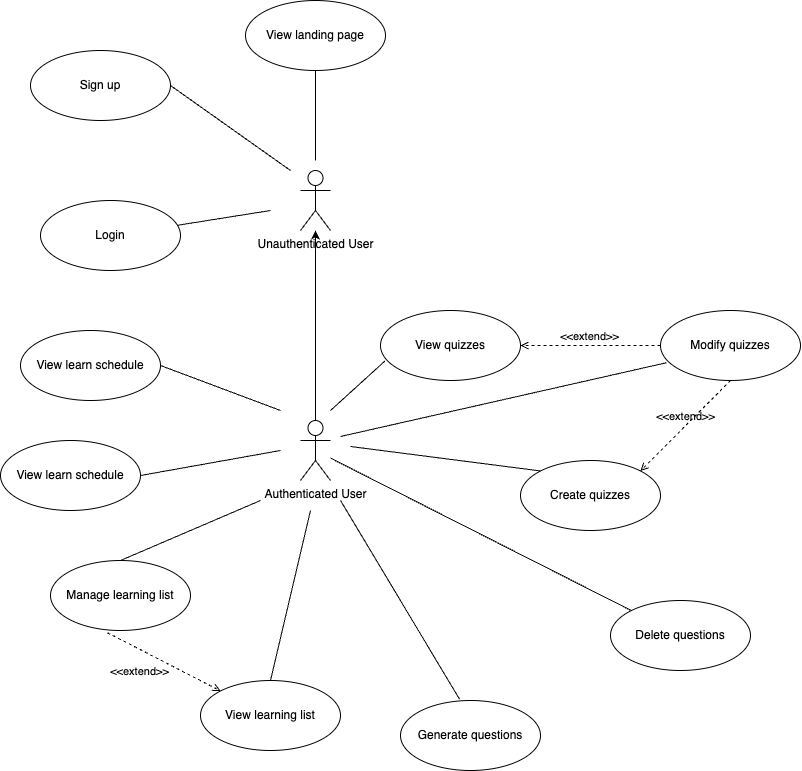
\includegraphics[width=0.8\textwidth, keepaspectratio]{figures/use-case.png}
    \caption{SpacedAce use case diagram}
    \label{fig:use-case}
\end{figure}

\subsection{Authentication}

The features are available after authentication, so the platform allows users to log in or create a new account with a simple form. Unauthenticated users can only view the landing page and authentication-related pages.

\subsection{Quizzes}\label{subsec:quizzes}

Authenticated users on the platform can list and view their quizzes. They can also create new quizzes by providing a name and a description, which can be modified later. Users can add and remove questions to their quizzes using the platform's question-generation feature.

Users can select quizzes to answer their questions. The platform lists all the questions in a column layout, while the users can answer them. It stores the answers so users can continue a started quiz later. After completing the users must submit their answers to the platform to review and score them. These results are shown after the quiz competition and can be seen in the \texttt{History page}.

\subsection{Questions}

As the previous subsection~\ref{subsec:quizzes} says, the users can add questions to quizzes or remove them. The large language model generates these questions by providing a text context and a question type. The context can be a few sentences long in any topic or numerous paragraphs. The platform chunks the long text contexts and uses them in smaller portions to generate more diverse questions.

The platform supports the following question types: single-choice, multiple-choice, and boolean. The single-choice questions have four possible answers, but exactly one is correct. The multiple-choice questions are similar, but multiple answers could be correct, even for all of them, but at least one. Boolean questions consist of a statement that can be true or false.

\subsection{Learning list}

Every user has a list of quizzes they would like to learn. This list is called the learning list. They can add quizzes to the list or remove ones already added. When a quiz is added to a user's learning list, the platform schedules the related questions to learn using the spaced ace algorithm. This function is available from the \texttt{My quizzes} page by clicking the \texttt{Learning list} button to show a learning list manager popup.

\subsection{Learn using spaced repetition}

The users can list the spaced repetition scheduled questions on the \textt{Learn} page. They can choose to review all of them by letting the platform show them after each other or review them individually.
